\section{Implementierung}

\subsection{OpenCL}

\subsubsection{Einleitung}

\begin{itemize}
\item CFD ist sehr anspruchsvoll was Rechenaufwand angeht
\item Traditionellerweise hat man (für Endanwender) auf CPUs programmiert
\item CPUs haben seit kurzem immerhin mehrere Kerne, sodass OpenMP und MPI Sinn ergeben
\item Die Entwicklung zu mehreren Kernen wurde von der Stromsparüberlegung angetrieben (viele Kerne mit niedrigeren Frequenzen leisten dasselbe, sind aber energieeffizienter)
\item Dadurch außerdem kleinere, spezialisiertere Prozessoren (weniger "wasted transistors")
\item Aber GPUs haben theoretisch wesentlich mehr Rechenpower\cite{Guide2012}
\item Grade CFD ist sauschnell
\item Aber natürlich brauch man Probleme, die gut parallelisierbar sind
\item Definition Concurrency: "A software system is concurrent when it consists of more than one stream of operations that are active and can make progress at one time."
\item Definition Parallelism: "When concurrent software runs on a computer with multiple processing elements so that threads actually run simultaneously, we have parallel computation. Concurrency enabled by hardware is parallelism."
\item In diesem Abschnitt Architektur von OpenCL deutlich machen und klären welche Probleme damit gut lösbar sind.
\end{itemize}

\subsubsection{Architektur}

\begin{itemize}
\item Dezember 2008 released
\item Momentan bei Version 1.2, obwohl das noch wenige implementieren
\end{itemize}

\begin{itemize}
\item Parallelisierbarkeit erklären: data parallelism und task parallelism
\item Dataparallelism: Idee ist, dass man eine Sammlung von Daten hat, die
nebenläufig upgedatet werden können. Parallelität wird nun grade dadurch
erzeugt, dass man denselben Instructionstream auf jedes Datenelement abfeuert
(nicht etwa für jedes Datenelement 'nen eigenen Thread hat, der sich beliebig
 anders verhält als der nächste Thread). Beispiel: Addition zweier Vektoren
(SIMD allgemein).
\item Taskparallelism: Eignet sich vielleicht eher für Traversierung von Graphen
oder so.
\item Platform-Model erklären
	\begin{itemize}
		\item "High level description of the heterogenous system"
		\item Host (gibt nur einen)
		\item Host enthält Devices
		\item Devices enthalten Compute Units
		\item Compute Units enthalten Processing Elements
		\item Host program, was auf Host läuft
		\item Mehrere Kernel laufen auf jeweils einem Device
		\item Execution Model klärt, wie Kernel ausgeführt werden
	\end{itemize}
\item Execution-Model
	\begin{itemize}
		\item "abstract representation of how streams of instructions execute on the heterogenous platform"
		\item Kernelexecution löst die Erstellung eines ganzzahligen "Gitters" aus, jeder Kernel kriegt eine Gitterzelle, die globale ID und wird zum "Work-Item"
		\item Workitems werden in Workgroups zusammengefasst (haben auch ID, bilden eine gröbere Struktur, haben geteilten Speicher, werden auf derselben Computeunit ausgeführt)
		\item Command-Queues, schedulen Kernel, Memorycommands, Synchronisierungskommandos, in-order, out-of-order
		\item Barrieren, Warps
	\end{itemize}
\item Memory-Model
	\begin{itemize}
		\item "the collection of memory regions withing OpenCL and how they interact during an OpenCL computation"
		\item Bufferobjects (eindimensional, beliebige Datentypen), Imageobjects, mehrdimensional usw., Inhalt "versteckt"
		\item Host memory
		\item Global, local, private, constant
		\item Zusammenspiel mit OpenGL
	\end{itemize}
\item Programming model
\begin{itemize}
	\item High level abstractions for algorithm programming
	\item OpenCL-C erläutern
\end{itemize}
\end{itemize}

\subsection{Schneesimulation}

\subsubsection{Allgemein}

Für die Simulation des Winds ist es wichtig, eine möglichst optimale
Datenstruktur zur Speicherung der verwendeten Felder zu verwenden, um
die Speicherzugriffszeiten zu minimieren und die maximale Performance zu
erreichen.

Wie bereits angesprochen bietet OpenCL zur Speicherung die Wahl zwischen Buffern
und Texturen (sofern Texturen auf der Zielplattform unterstützt werden). Beide
Speicher-Arten haben leicht unterschiedliche Anwendungsgebiete. In vielen
Kerneln sind wir daran interessiert, für die \PimiddyQuotes{aktuelle} Zelle den
Wert des Gitters sowie den Wert aller Nachbarn zu bestimmen, wobei der
\PimiddyQuotes{Wert} je nach Feld-Typ entweder Druck, Geschwindigkeit oder etwas
anderes bedeuten kann. Außerdem wird bei der Advektion linear zwischen Voxeln
interpoliert.

Schnelle Zugriffe auf einen Voxel samt seiner Nachbarn sind ein Merkmal von
Texturen, daher würden sie sich für viele Kernel anbieten. Allerdings ist das
Schreiben von 3D-Texturen in OpenCL-1.1 nur mit einer Extension möglich. Als
Hilfsmaßnahme greift man hier üblicherweise zu sogenannten
\PimiddyBegriff{Flat-3D-Texturen} \cite{Harris2003}. Hier werden die einzelnen
\PimiddyQuotes{Scheiben} der dreidimensionalen Struktur nebeneinander in eine
zweidimensionale Textur geschrieben, siehe
\autoref{fig:implementation_flat_3d_texture}. Für die Umrechung zwischen 3D- und
2D-Koordinaten ist etwas Rechenaufwand nötig. 2D-Texturen erlauben außerdem
natürlicherweise nur zweidimensionale Interpolation. Benötigt man
dreidimensionale Interpolation, ist auch hier etwas Mehraufwand zu verrechnen.
Texturen werden optimiert gespeichert, sodass Leseoperationen beschleunigt
werden. Diese optimierte Speicherung führt aber dazu, dass das Schreiben in
Texturen relativ langsam ist. Benchmarks im Zweidimensionalen bestätigten, dass
Buffer tatsächlich schneller sind.

\begin{figure}[ht]
\centering
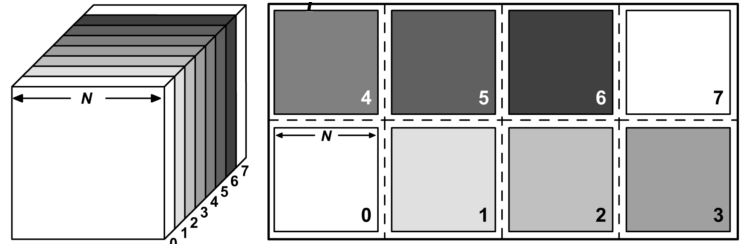
\includegraphics[width=8cm]{images/flat_3d_texture}
\caption{Veranschaulichung einer Flat-3D-Textur}
\label{fig:implementation_flat_3d_texture}
\end{figure}

Da Buffer eindimensional sind, muss zwischen drei- und eindimensionalen
Koordinaten konvertiert werden. Sei $(x,y,z)$ eine dreidimensionale Koordinate
und $(w,h,d)$ die Dimensionen eines Buffers (er enthält also $w \cdot h \cdot d$
Elemente). Dann erhält man den eindimensionalen Index mittels:

\begin{equation}
i = w \cdot h \cdot z + w \cdot y + x
\end{equation}

Umgekehrt erhält man die $(x,y,z)$-Koordinaten eines Index mittels

\begin{align*}
x &= i \PimiddyModulo w \\
y &= i \PimiddyModulo w \cdot h \\
z &= i / (w \cdot h)  \\
\end{align*}

Im Weiteren wird das Verfahren von Stam in OpenCL umgesetzt. Dabei wird auf
Besonderheiten in der Implementierung eingegangen. Fast alle Kernel greifen
hierbei auf den Buffer zurück, der die Hindernisinformationen enthält. Wie
dieser Buffer gefüllt wird, wird im letzten Abschnitt erläutert.

\subsubsection{Verfahren nach Stam in OpenCL}

Gegeben sei ein Buffer \PimiddyInlineCode{boundaries} vom Typ
\PimiddyInlineCode{float}, der 1.0 enthält, wenn die zugehörige Gitterzelle ein
Hindernis enthält und 0.0 wenn nicht. Außerdem gegeben sei ein Buffer
\PimiddyInlineCode{velocity} vom Typ \PimiddyInlineCode{float4}, der das
momentane Geschwindigkeitsfeld enthält. Dieses Feld wird anfangs auf $(0,0,0,0)$
gesetzt. Der Wind wird manuell von einer Seite in die Simulation gespeist und
breitet sich dann aus. Viele der Algorithmen benötigen außerdem das Zeitdelta
\PimiddyInlineCode{float dt}.

Der erste Schritt im Verfahren nach Stam ist die Advektion des Vektorfeldes
\PimiddyInlineCode{velocity}. Der dazugehörige Kernel ist aus mehreren
Funktionen zusammengesetzt. Zunächst benötigen wir eine Struktur, um die
Nachbarn des aktuellen Punktes zu speichern:





\begin{itemize}
\item Erklärung der Algorithmen mit (Pseudo?)-Code
\item Zuerst Advektion. Hier ansprechen, dass vielleicht Texturen besser wären
wegen "random gather" und Interpolation, aber dazu Umkonvertierung
\item Dann Jacobiverfahren, hier vor allem Pingpong zwischen Buffern erklären
und wie viele Iterationen man machen muss/kann.
\item Dann Subtraktion des Gradienten
\item Hindernisse, Visualisierung (Laden aus obj-Datei)
\item Hindernisse, Voxelisierung mit binvox (Quelle \cite{Nooruddin2003}, \cite{binvox2012}
\end{itemize}

\subsection{Fliegender Schnee}

\begin{itemize}
\item Grundsätzliche Einteilung
	\begin{itemize}
	\item Kurze Einführung wo Schnee herkommt
	\item Aussehen der Schneeflocken
	\item Simulation der Schneeflocken, erst Physikalisch
	\item Dann, wenn nötige Eigenschaften bekannt sind, Partikelsystem erklären
	\end{itemize}
\item Niederschlag erklären: Luft im Himmel ist mit Wasser gesättigt, das
gesättigte Wasser kondensiert zu Tropfen, Tropfen wachsen bis sie
herunterfallen. Tropfen bilden sich nur, wenn Kondensationskerne (wie Staub) in
der Luft sind, an die das Wasser sich anheften kann.
\item Schneefall: Temparatur muss kleiner 0 Grad sein. Kondensationskerne müssen
eine gewisse Form haben (wird bei $<-40$ Grad unnötig)
\item Schneeflocken haben sehr vielfältige Formen und Größen (Entstehung dieser Formen kurz erklären?)
\item Werden visuell vereinfacht zu Point Sprites
\item Point Sprites Punkte mit Ausdehnung und Textur, zeigen immer zum
Betrachter, Größe selber festlegbar, abhängig von der Kamera, Bild wird atlased
und je nach Flockeneigenschaft (bzw. Temparatur der Umgebung) ausgewählt
\item Physikalische Eigenschaften einer Schneeflocke
\item Kräfte sind gravity, buoyant, lift und drag.
\item Drag ist die Kraft, die die Schneeflocke entlang des Wind treiben lässt
\item Lift lässt die Flocke in Kreisförmigen Bewegungen runterfallen
\item Drag ist definiert durch
\[
F_{drag} = \frac{1}{2} \rho_{air} \vec{U}_{fluid}^2 A C_D
\]
wobei $\rho$ die Dichte der Luft angibt, $U$ die
Geschwindigkeit, $A$ der Durchmesser, $C_D$ der Drag-Koeffizient, der auf die
Form der Schneeflocke ankommt und die Turbulenzen die sie erzeugt.
\item Angenommen die Schneeflocke hat eine bestimmte Masse und fällt mit
terminal velocity nach unten, dann kann man $C_D$ bestimmen (abhängig von $U_{max}, \rho, A, m_{snow}$
\item Das kann man in $F_{drag}$ einsetzen und erhält
\[
F_{drag} = \frac{U_{fluid} m_{snow} g}{U_{max}}
\]
\item Man muss also nur $U_{max}$ schätzen. In \cite{Hanesch1966} wurde das
gemacht (bei -2 bis 0 Grad Celsius). Feststellung: Größe der Schneeflocke hat
kaum Einfluss. Geschwindigkeit ist zwischen $0.5m/s$ und $2m/s$. In
\cite{Canada1999} wurde zudem festgestellt, dass zwischen trockenem Schnee und
nassem Schnee ein Faktor von 2 ergibt, d.h. nasser Schnee hat $1-4m/s$ und
trockener eben $0.5-2$
\item Lift force ist orthogonal zur Dragforce und entsteht durch vortex shedding
hinter der Schneeflocke. Flocke wird zur Seite abgetrieben.
\item Via Weg-Zeit-Gesetz:
\[
s=\frac{1}{2}at^2 + v_0 t + s_0
\]
Berechnen wir die neue Position eine Schneeflocke via:
\[
\vec{p}^{t+\Delta t} = \vec{p}^t + \vec{u} \Delta t + \frac{1}{2} \vec{a} \Delta t^2
\]
D.h. wir speichern eine Geschwindigkeit und Berechnen eine (konstante) Beschleunigung

\textbf{Alternativ}: Schlicht zwei DGL hinschreiben:
\begin{gather}
p^{t + \Delta t} = p^{t} + \Delta t \cdot \vec{u}^{t} \\
\vec{u}^{t+ \Delta t} = \vec{u}^{t} + \Delta t \cdot \vec{a}^{t} \\
\vec{a}^t = \frac{\vec{F}_{ges}}{m_{snow}}
\end{gather}
\item Erste Kraft, Gravitation
\item Zweite Kraft, Auftrieb, wird aber vernachlässigt
\item $F_{lift}$ erzeugt spiralförmige Bewegung, allerdings relativ subtil. Wird angenähert durch:
\[
U_{circ} = C_{vel} \omega (\sin(\omega t),0,\cos(\omega t))
\]
\item Erstmal weglassen
\item Nötige Eigenschaften einer Schneeflocke: Position, Geschwindigkeit (dynamisch), Masse (für Drag), Maximalgeschwindigkeit $U_{max}$.
\item Simulation vom Aufbau her:
	\begin{itemize}
		\item Generiere Zufallswerte für Schneeflockenposition-,
		Geschwindigkeit, Masse, Maximalgeschwindigkeit, Bild
		\item In jedem Frame update Geschwindigkeit und Position
		\item Teste auf Hindernis, falls erfolgreich, generiere neue
		Zufallsposition (oder wenn Schneeflocke außerhalb ist)
		\item Update ggf. die Schneeaktivität.
	\end{itemize}
\item Simulation in Code, Buffersharing mit OpenGL, Shader in OpenG.
\end{itemize}

\subsection{Liegengebliebener Schnee}

\begin{itemize}
\item Marching Cubes, allgemeine Beschreibung
\item Marching Cubes auf der GPU
\item Zusammenhang mit Schneemodell
\item Triplanare bzw. prozedurale Texturierung
\end{itemize}

\subsection{Andere Visualisierungsmöglichkeiten}

\begin{itemize}
\item Rauch
\end{itemize}
